\documentclass[11pt, a4paper]{article}
\usepackage{geometry}
\geometry{top=1.8cm,bottom=1.5cm,left=0.5cm,right=0.5cm, a4paper}
\usepackage{tikz}
\usetikzlibrary{positioning, arrows.meta}
\usepackage[many]{tcolorbox}
\usepackage{ragged2e}

% For a box
\newtcolorbox{boxing}{
    colback = pink!20, 
    colframe = pink!70, 
    boxrule = 0pt, 
    leftrule = 6pt,
    width=0.25\paperwidth
}


%  #1 -- Legend name
%  #2 -- Color

\newcommand{\drawLegends}[2]{
    \centering
    \begin{tikzpicture}[baseline=(label.base)]
        \node[circle, draw, inner sep=3.5pt, fill=#2] (label) {\textcolor{#2}{1}};
    \end{tikzpicture}
    #1
    \hspace{0.4cm}
}

\def \circledetails{
    \centering
    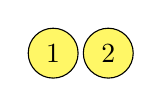
\begin{tikzpicture}[baseline=(label.base)]
        \node[circle, draw, inner sep=3.5pt, fill=yellow!60] (label) {1};
        \node[circle, draw, inner sep=3.5pt,xshift=7mm, fill=yellow!60] (label) {2};
    \end{tikzpicture}
    \hspace{0.4cm}
    1. Class average
    \hspace{0.2cm}
    2. No.of students below 50\%
}


% #1 -- space between the chart and legend
% #2 -- space between the legends 
% #3 -- Student count

\newcommand{\flowchartDescription}[3]{

  \vspace{#1cm}
  \begin{minipage}{0.6\linewidth}
    \drawLegends{Above 80\%}{green!50}
    \drawLegends{Between 60\% and 80\%}{blue!30}
    \drawLegends{Below 60\%}{yellow!60}

    \vspace{#2cm}
    \circledetails
  \end{minipage}
  \begin{minipage}{0.3\linewidth}
    \RaggedLeft{ \begin{boxing}
      Total No.of Students: \textbf{#3}
      \end{boxing} }
  \end{minipage}

}

\begin{document}

\small
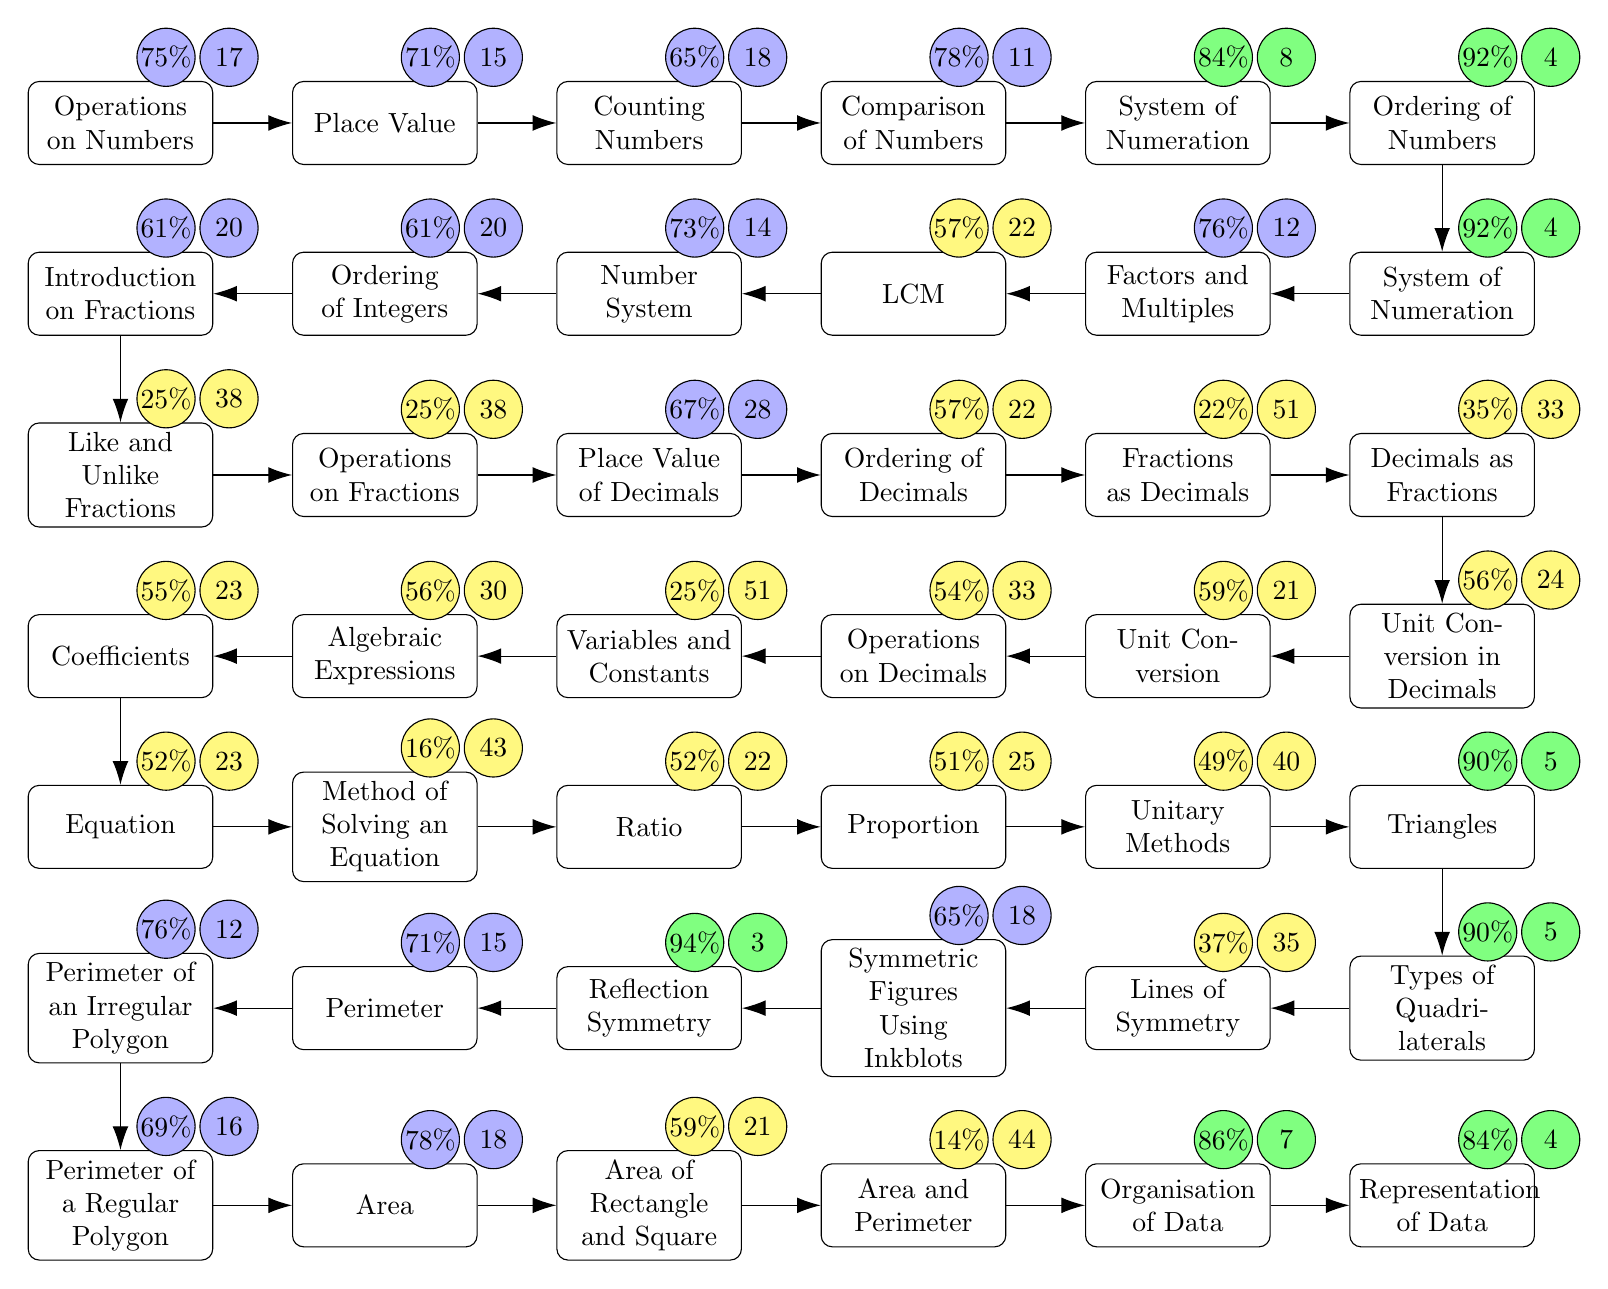
\begin{tikzpicture}[
    % Styles for the nodes and lines
    block/.style={rectangle, draw, text width=6em, text centered, rounded corners, minimum height=3em},
    node distance=1.1cm and 1cm, % Adjusting the distance between the nodes
    line/.style={
        draw, 
        -{Latex[length=3mm,width=2mm]}
    },
    ring/.style={
        circle,
        draw,
        inner sep=0pt,
        minimum size=2.1em % Increased from 2em to 3em for a slightly larger ring
    },
    ringhighlightyellow/.style={ % Style for highlighted ring in yellow
        ring,
        fill=yellow!50, % Fill color set to yellow with 50% opacity
        minimum size=2.1em
    },
    ringhighlightblue/.style={ % Style for highlighted ring in blue
        ring,
        fill=blue!30, % Fill color set to blue with 30% opacity
        minimum size=2.1em
    },
    ringhighlightgreen/.style={ % Style for highlighted ring in green
        ring,
        fill=green!50, % Fill color set to green with 50% opacity
        minimum size=2.1em
    }
]

% Initialize a counter to keep track of the last node created
\newcounter{nodecounter}
\setcounter{nodecounter}{0}

% Define a new command to create a node connected from the previous node with an additional parameter for the percentage
\newcommand{\connectnodes}[4]{
    % Increment node counter
    \stepcounter{nodecounter}
    
    % Check if it's the first node to determine positioning
    \ifnum\value{nodecounter}=1
        \node [block] (\arabic{nodecounter}) {#4}; % Place the first node without positioning
    \else
        % Calculate the previous node's number
        \pgfmathtruncatemacro{\prevnode}{\value{nodecounter}-1}
        \node [block, #3=of \prevnode] (\arabic{nodecounter}) {#4}; % Position based on direction and previous node
        % Draw the line from the previous node to the current node
        \path [line] (\prevnode) -- (\arabic{nodecounter});
    \fi
    
    % Determine the ring style based on the percentage
    \pgfmathparse{#2<60?"ringhighlightyellow":(#2<=80?"ringhighlightblue":"ringhighlightgreen")}
    \edef\ringstyle{\pgfmathresult}
    
    % Draw the rings with percentage symbol
    \node [\ringstyle] at ([xshift=2mm,yshift=3mm]\arabic{nodecounter}.north east)  {#1}; % 'ring-count' with an xshift and yshift
    \node [\ringstyle] at ([xshift=-6mm,yshift=3mm]\arabic{nodecounter}.north east) {#2\%}; % New ring with the percentage to the left of the 'ring-count', now includes % symbol
}




% Create nodes and paths with the new command structure. The second parameter is now the percentage displayed in the ring to the left.
\connectnodes{17}{75}{right}{Operations on Numbers};
\connectnodes{15}{71}{right}{Place Value};
\connectnodes{18}{65}{right}{Counting Numbers};
\connectnodes{11}{78}{right}{Comparison of Numbers};
\connectnodes{8}{84}{right}{System of Numeration};
\connectnodes{4}{92}{right}{Ordering of Numbers};
\connectnodes{4}{92}{below}{System of Numeration};
\connectnodes{12}{76}{left}{Factors and Multiples};
\connectnodes{22}{57}{left}{LCM};
\connectnodes{14}{73}{left}{Number System};
\connectnodes{20}{61}{left}{Ordering of Integers};
\connectnodes{20}{61}{left}{Introduction on Fractions};
\connectnodes{38}{25}{below}{Like and Unlike Fractions};
\connectnodes{38}{25}{right}{Operations on Fractions};
\connectnodes{28}{67}{right}{Place Value of Decimals};
\connectnodes{22}{57}{right}{Ordering of Decimals};
\connectnodes{51}{22}{right}{Fractions as Decimals};
\connectnodes{33}{35}{right}{Decimals as Fractions};
\connectnodes{24}{56}{below}{Unit Conversion in Decimals};
\connectnodes{21}{59}{left}{Unit Conversion};
\connectnodes{33}{54}{left}{Operations on Decimals};
\connectnodes{51}{25}{left}{Variables and Constants};
\connectnodes{30}{56}{left}{Algebraic Expressions};
\connectnodes{23}{55}{left}{Coefficients};
\connectnodes{23}{52}{below}{Equation};
\connectnodes{43}{16}{right}{Method of Solving an Equation};
\connectnodes{22}{52}{right}{Ratio};
\connectnodes{25}{51}{right}{Proportion};
\connectnodes{40}{49}{right}{Unitary Methods};
\connectnodes{5}{90}{right}{Triangles};
\connectnodes{5}{90}{below}{Types of Quadrilaterals};
\connectnodes{35}{37}{left}{Lines of Symmetry};
\connectnodes{18}{65}{left}{Symmetric Figures Using Inkblots};
\connectnodes{3}{94}{left}{Reflection Symmetry};
\connectnodes{15}{71}{left}{Perimeter};
\connectnodes{12}{76}{left}{Perimeter of an Irregular Polygon};
\connectnodes{16}{69}{below}{Perimeter of a Regular Polygon};
\connectnodes{18}{78}{right}{Area};
\connectnodes{21}{59}{right}{Area of Rectangle and Square};
\connectnodes{44}{14}{right}{Area and Perimeter};
\connectnodes{7}{86}{right}{Organisation of Data};
\connectnodes{4}{84}{right}{Representation of Data};


\end{tikzpicture}

\flowchartDescription{2}{1}{90}

\end{document}